\documentclass[conference]{IEEEtran}
\IEEEoverridecommandlockouts
% The preceding line is only needed to identify funding in the first footnote. If that is unneeded, please comment it out.
\usepackage{cite}
\usepackage{amsmath,amssymb,amsfonts}
\usepackage{algorithmic}
\usepackage{graphicx}
\usepackage{textcomp}
\usepackage{xcolor}
\usepackage{comment}
\def\BibTeX{{\rm B\kern-.05em{\sc i\kern-.025em b}\kern-.08em
    T\kern-.1667em\lower.7ex\hbox{E}\kern-.125emX}}
\begin{document}

\title{Lung Cancer Classification from Whole slide Histopathological Images using Deep Learning Techniques}



\author{\IEEEauthorblockN{P. Mirunalini\IEEEauthorrefmark{1},
S. Pavya\IEEEauthorrefmark{2}, N. Priyadharshini \IEEEauthorrefmark{3} and Karthik D\IEEEauthorrefmark{4}}
\IEEEauthorblockA{Dept. of Computer Science\\
SSN College of Engineering\\ Chennai, India\\
Email: \IEEEauthorrefmark{1}miruna@ssn.edu.in,
\IEEEauthorrefmark{2}pavya17102@cse.ssn.edu.in ,
\IEEEauthorrefmark{3}priyadharshini17118@cse.ssn.edu.in ,\\
\IEEEauthorrefmark{4}karthik19047@cse.ssn.edu.in,
 }}


\begin{comment}
\author{\IEEEauthorblockN{P. Mirunalini}
\IEEEauthorblockA{\textit{Dept. of Computer Science} \\
\textit{SSN College of Engineering}\\
Chennai, India}

\and 

\IEEEauthorblockN{S. Pavya}
\IEEEauthorblockA{\textit{Dept. of Computer Science} \\
\textit{SSN College of Engineering}\\
Chennai, India}
\and

\IEEEauthorblockN{N. Priyadharshini}
\IEEEauthorblockA{\textit{Dept. of Computer Science} \\
\textit{SSN College of Engineering}\\
Chennai, India}

\and
\IEEEauthorblockN{Karthik D}
\IEEEauthorblockA{\textit{Dept. of Computer Science} \\
\textit{SSN College of Engineering}\\
Chennai, India}

}
\end{comment}

\maketitle

\begin{abstract}
Lung Cancer is a leading cause of death worldwide, Which begins in lungs and may spread to lymph nodes or other organs in the body. There are several types of lung cancer among them adenocarcinoma, benign and squamous cell carcinoma are more prevailing hence diagnosis and treatment of lung cancer is very much needed to known about the cancer type. Automated detection of cancer types would significantly speed up the diagnosis and treatment. So we propose two different methods to classify the lung cancer types using Deep learning techniques. In our first method we proposed a Convolutional Neural Network(CNN) to classify the lung cancer types from the whole slide histopathological images and attained an accuracy of 99\%. The cancer mainly affects the nucleus of the tissues, so in our second method we performed the classification of lung cancer types from the segmented nuclei. The nuclei were segmented from the whole slide histopathological images using threshold based and color based methods. The segmented nuclei were classified using CNN and achieved an accuracy of 99\%. We have performed many experiments and evaluated the proposed methods at each level.

\end{abstract}

\begin{IEEEkeywords}
Segmentation, Histopathological Images, Adenocarcinoma, Squamous Cell Carcinoma, Benign, Deep learning, Convolutional Layer
\end{IEEEkeywords}

\section{Introduction}
\subsection{Lung Cancer Types And Causes}
 Taking in oxygen and getting rid of carbon dioxide is the main function of lung. If lung cells grow and multiply uncontrollably, tumors may develop. Tumors that are composed of normal lung cells are termed as a benign tumor. On the other hand, if they are made up of cancerous cells that could spread to other tissues, the tumor is said to be malignant.  Lung cancer occurs in parts of the lungs such as bronchi, bronchioles or alveoli. There are many factors that may cause lung cancer. The most common causes of lung cancer are smoking and exposure to secondhand smoke. Lung cancer in non-smokers is mainly due to gene changes or workplace exposure to asbestos, diesel exhaust and certain other chemicals. 
\newblock
\begin{figure}[htbp]
\centerline{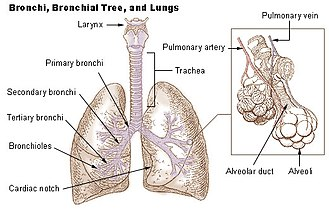
\includegraphics[width=7cm,height=5cm]{./figures/fig1.jpg}}
\caption{Lung Structure}
\label{fig1}
\end{figure}
The tumors can either be cancerous(malignant) or non-cancerous(benign) as shown in figure \ref{fig2}
\begin{figure}[htbp]
\centerline{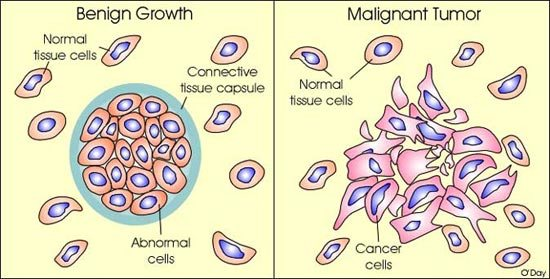
\includegraphics[width=7cm,height=5cm]{./figures/fig2.jpg}}
\caption{Malignant and Benign type cells}
\label{fig2}
\end{figure}

\subsection{Imaging Modalities}
There are different imaging modalities to detect lung cancer such as CT scan, MRI scan and histopathological images. Repeated exposure to radiation and injection of contrast agents during CT and MRI imaging can have adverse effects on the patient's health. The histopathological imaging procedure is a relatively safer modality when compared to other modalities. The term histopathology refers to the study of tissues characteristics which is performed by analysing blood samples of the tissues. Histopathological examination is considered as a gold-standard since it helps in accurate diagnosis and sub-typing of lung lesions \cite{histo_study_lungbiopsy}. It also helps in distinguishing between lesions not only during the detection and but also during follow-ups and also helps in the prognostication and treatment decisions \cite{histopath_role}. 

Images acquired by histopathology contains biopsy of the affected tissues. These tissues are stained with hematoxylin and eosin and further examined under a microscope to detect malignant features in the cellular structures such as the nuclei. Nuclei can exhibit a wide variety of patterns that are diagnostically significant. The appearance of the nuclei may be different due to factors such as nucleus type, malignancy of the disease and the nuclei life cycle. Non pathological epithelial nuclei (EN) have uniform chromatin distribution with smooth boundary whereas,  pathological EN are larger in size and have a heterogeneous chromatin distribution, irregular boundaries\cite{irshad}. Thus, analysing the nucleus will help in detecting the cancerous tumors. In order to analyse the histopatholgical images, the nuclei can be segmented and used for further analyse to detect the cancerous cells.

Manual detection of a cancer cell from histopathological images is a time-consuming as the cells are irregular and arbitrary visual angles. It also involves inter and intra-observer variability\cite{sumaiya}. Hence, an automated system can help in quick diagnosis. This automation can be achieved through machine learning systems. The accuracy of the system purely depends on feature engineering. In order to overcome the aforementioned problems, we propose to develop an automated deep learning system to analyse the histopathological images of the lungs and detect the presence of cancerous cells, using different techniques. The ultimate goal of the proposed system is to identify whether the tumor is benign or malignant as malignant cells, if not treated immediately, can prove to be fatal.

The sample histopathological images are shown in Figure \ref{histo_img}
\begin{figure}[htbp]
\centerline{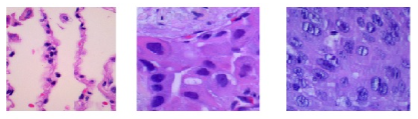
\includegraphics[width=8cm, height=4cm]{./figures/histo_img.png}}
\caption{Histopathological Images}
\label{histo_img}
\end{figure}
 Most of the literature use CNN for lung cancer classification system and digital pathology plays a  major role in lung cancer treatment \cite{wang2019artificial}. Deep Convolution Neural Network(DCNN) based feature learning is proposed \cite{xu2016deep} to automatically classify EP and ST regions from digitized tumor tissue micro-arrays. Deep learning convolutional neural network (CNN) model (inception v3) on histopathology images obtained from the Cancer Genome Atlas (TCGA) is proposed \cite{coudray2018classification} to accurately classify whole-slide pathology images into adenocarcinoma, squamous cell carcinoma or normal lung tissue. An automated classification scheme for lung cancers presented in microscopic images using a deep convolutional neural network (DCNN) was proposed \cite{teramoto2017automated} to classify three types of lung cancer(Adenocarcinoma, squamous cell carcinoma, small cell carcinoma). A deep learning framework is proposed \cite{grahamaclassification} to classify the input patches into adenocarcinoma and squamous cell carcinoma. An automated cell type classification pipeline,ConvPath \cite{wang2019convpath} which includes nuclei segmentation, convolutional neural network-based tumor cell, stromal cell, and lymphocyte classification and extraction of tumor micro-environment-related features for lung cancer pathology images.
 
 
\section{Proposed System}
We have proposed two different automated methods to classify tumors as benign and malignant. In our first method we have used a deep learning technique to classify the whole slide histopathological images and our second method we have segmented the nucleus and classified the segmented nuclei using deep learning techniques. We have also performed experiments to achieve two different types of classification - a binary classification of tumors into benign and malignant and a multi class classification of malignant tumors into its subtypes as adenocarcinoma and squamous cell carcinoma and benign tumors
\begin{comment}
\begin{enumerate}
  \item Lung cancer classification from whole slide histopathological images using deep learning.
  \item Lung cancer classification from segmented nuclei using deep learning.
\end{enumerate}
\end{comment}


\The architecture diagram of the proposed system is shown in figure \ref{Proposed System}
\begin{figure}[htbp]
\centerline{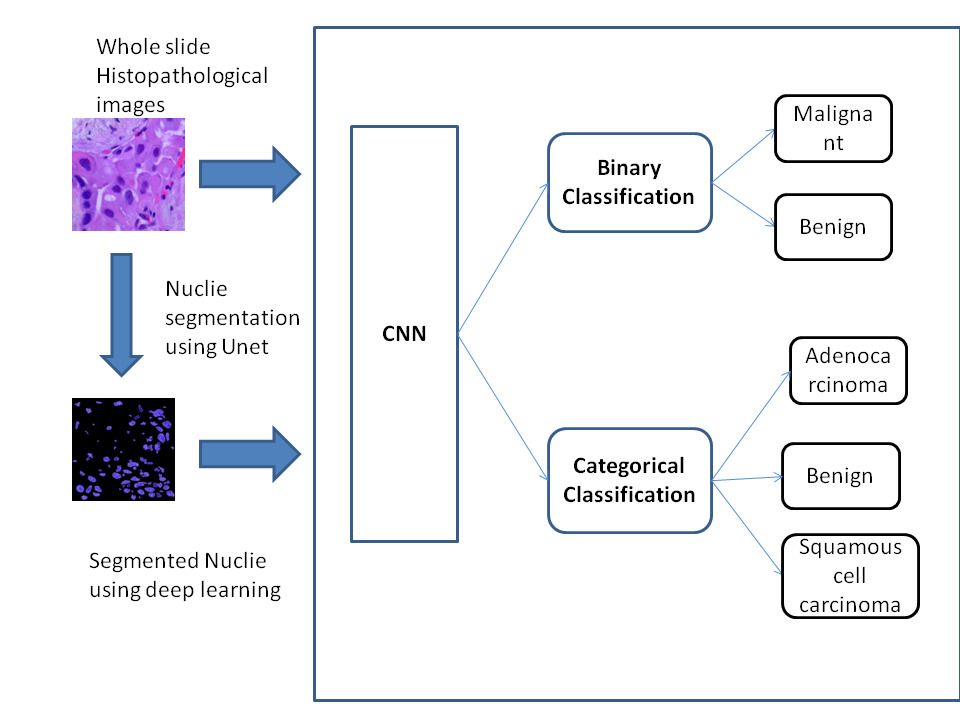
\includegraphics[width=9cm, height=8cm]{./figures/paper_proposed_sys.png}}
\caption{Proposed system}
\label{Proposed System}
\end{figure}

\subsection{Classification Of Lung Cancer From Whole Slide histopathological Images Using Deep Learning}

In our proposed work we classify the whole slide histopathological images using  Convolution Neural Network (CNN) a deep learning model. The histopathological images are made up of  different structures such as the nucleus, chromosomes, cytoplasm, lymphocytes etc. The deep learning model needs to learn features from the images, so it is necessary to have large amount of images. We have used a data augmentation technique that helps to generate more images by applying different transformation technique such as rotation, flipping and zooming on the input images. We have  generated images by performing  the rotation range of 20 degrees, zoom range as 0.05, height shift range and width shift range as 0.1, horizontal flip, vertical flip and random flip.

\subsubsection{CNN}
In our model, we have used six convolution layers, six max pooling layers and two dense layers. Out of the six layers each consists of a convolution followed by activation layer, batch normalization layer and max-pooling layer. After extracting the different features from the images using each layers the feature representation vectors are flattened using the flatten layer and fed into the classification layer. The classification layer consists of two dense  stages. The first stage includes a dense layer followed by activation and dropout layers. The second stage, where the actual classification occurs, includes a dense layer followed by an activation layer.

We have used a 2D separable convolution layer with a filter size of 32, kernel size of 3x3 and a stride length of 1. It performs channel-wise spatial convolution followed by a point- wise convolution, mixing the output channels.  Rectified Linear Unit (ReLU) function is used to activate the hidden layers while the Softmax function is used for the dense layers. The model is fed with 32 input images per batch and trained using the NAdam optimizer with a learning rate of 0.001. The dropout layers have a dropout rate of 0.25 in the hidden layers and 0.50 in the dense layers. We have conducted experiments to perform both binary classification as well as multi-class classification.

\subsection{Lung Cancer Classification From The Segmented Nuclei Using Deep Learning}

\begin{comment}
The binary classification and categorical classification of lung cancer types from the segmented nuclei is shown in Figure \ref{binary} and Figure \ref{categorical}.
\begin{figure}[htbp]
\centerline{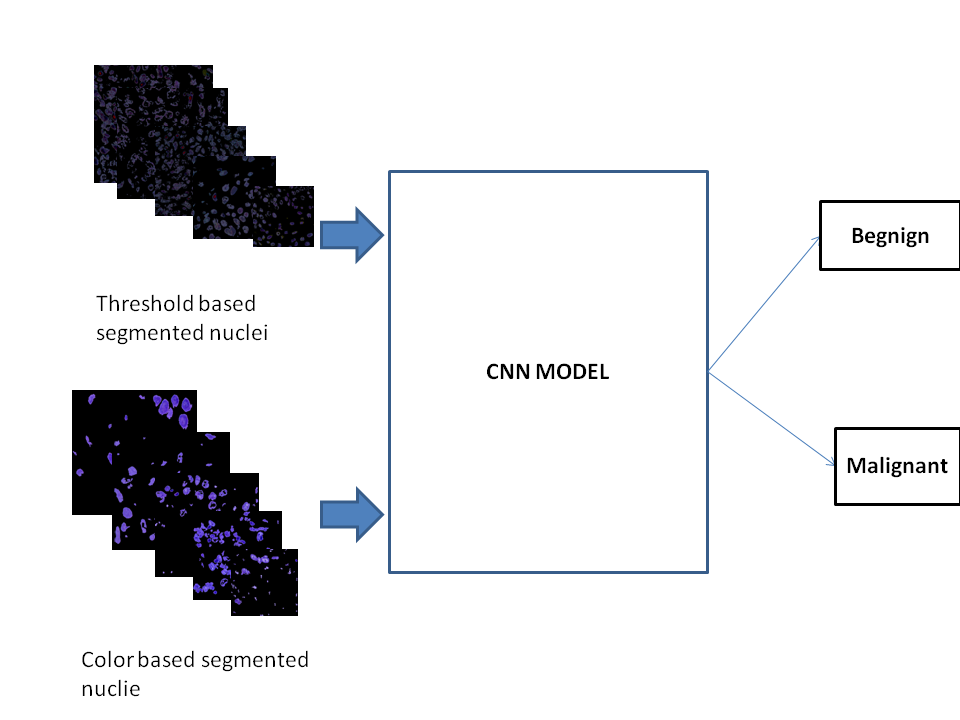
\includegraphics[width=8cm, height=7cm]{./figures/binary.png}}
\caption{Binary classification of lung cancer types from the segmented nuclei}
\label{binary}
\end{figure}
\begin{figure}[htbp]
\centerline{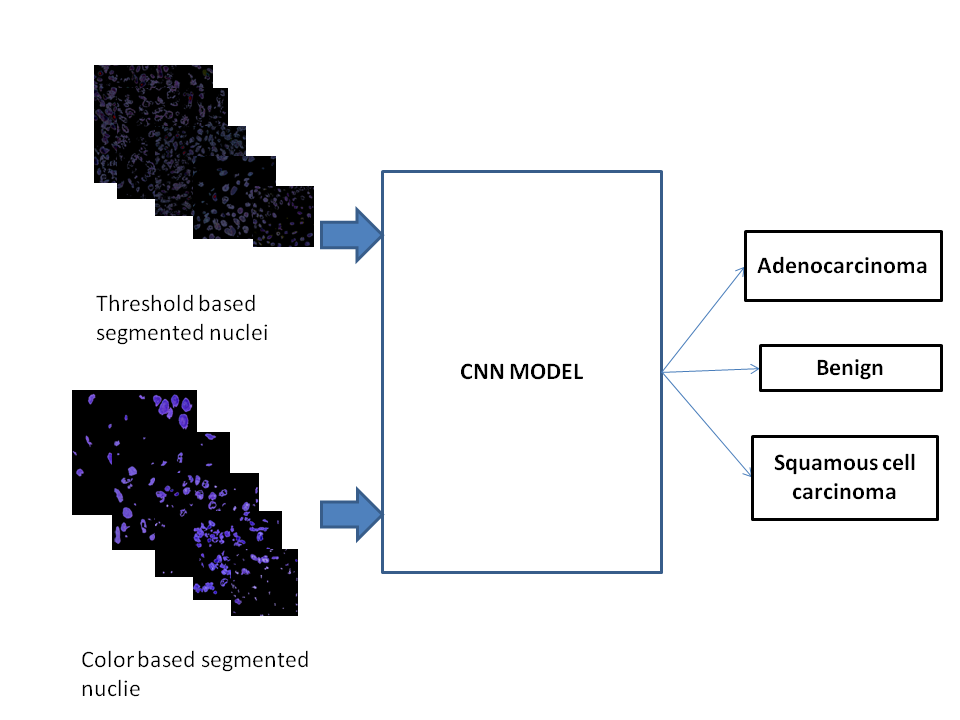
\includegraphics[width=10cm, height=7cm]{./figures/categorical.png}}
\caption{Categorical classification of lung cancer types from the segmented nuclei}
\label{categorical}
\end{figure}
\end{comment}


Nuclei segmentation in histopathology images using deep neural networks


\subsubsection{Nucleus Segmentation From Whole Slide Histopathological Images}
The Nucleus is segmented from the histopathological image tissues to do lung cancer classification based on the nucleus. The Nucleus is segmented from the histopathological images, because the nuclei are mainly affected by cancer. The structure of affected nucleus vary from normal one because of the nucleus mutation. By performing nuclei segmentation the cancer can be identified in the starting stage. The nuclei are segmented from the histopathological images using two methods one is using threshold based method and other one is using color based method. The advantage of color based method over threshold based method is the unwanted stains are removed in the color based segmentation.

\subsubsection{Classification On Threshold Based Segmented Nucleus}
In the threshold based segmentation the RGB image is converted into a gray-scale image in order to create the mask of the image. The mask of the gray-scale image is created by using the {\bf cv2.threshold()} operation. The threshold that we are using here is simple thresholding. That is, if the pixel value is smaller than the threshold it is set to 0, otherwise it is set to maxval(In our model it is 255).The threshold value that we have used for our model is 110 and the maxval is 100. The binary image is converted into a 3 channel image. This is done by using {\bf cv2.cvtColor()}. Then the {\bf cv2.bitwise\_and} operation (Figure \ref{result}) is performed between the 3 channel mask and the BGR image.
\begin{figure}[htbp]
\centerline{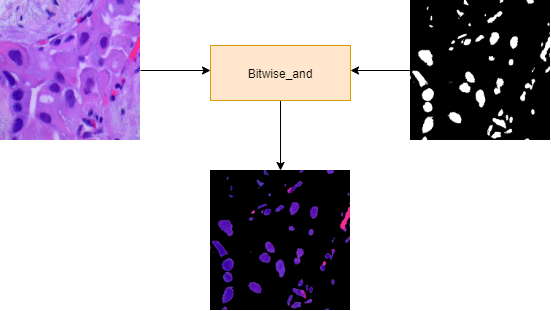
\includegraphics[width=8cm, height=5cm]{./figures/result.png}}
\caption{Bitwise And Operation}
\label{result}
\end{figure}
The segmented nuclei are obtained by performing the above operations (Figure \ref{threseg}) which is used for further classification.
\newline
\begin{figure}[htbp]
\centerline{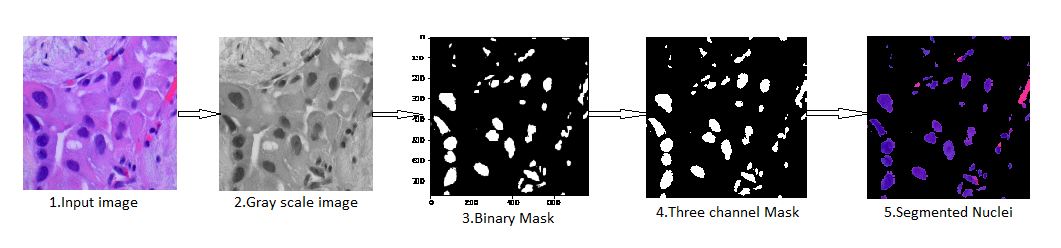
\includegraphics[width=10cm, height=4cm]{./figures/threseg.png}}
\caption{Threshold based Segmentation}
\label{threseg}
\end{figure}


\subsection{Histopathological Images}
 A histopathological image contains different parts such as the nucleus, chromosomes, etc. The nucleus is stained using Hematoxylin, which colors them blue or dark-purple, along with a few other tissues, such as keratohyalin granules and calcified material. Eosin stains the cytoplasm and some other structures including extracellular matrix such as collagen in up to five shades of pink
 and the other parts are stained using eosin. The purple colored part in the Figure \ref{histo_img} is the nucleus of the tissue sample, which is mainly affected by cancer.
{\bf Classification}
The proposed binary classification system classifies the lung cancer types into malignant and benign from the threshold based segmented nuclei (Figure \ref{binary}) and the categorical classification system (Figure \ref{categorical}) classifies the lung cancer types into adenocarcinoma, squamous cell carcinoma and benign type cells from the threshold based segmented nuclei.

\subsubsection{Classification On Color Based Segmented Nucleus}
In the color based nucleus segmentation the RGB image is converted into a gray-scale image in order to create the mask of the image. Also the RGB image is converted into HSV image, in order to find the average hue value of the nucleus. The binary mask of the gray-scale image is created using the threshold operation. The threshold value that we have used is 110 and the max\_val is 255. The contours of the binary mask is found. The contours are drawn in the empty mask. The nucleus of cancer cells in histopathological images are found to be in purple color. The average hue value for purple color is 154 to 170. The contours are filled with the nucleus from the original image if the hue value of the image lies between the given given range. Thus we obtained the segmented nucleus by performing above operations which is used for further classification.

{\bf Classification}
The proposed binary classification system (Figure \ref{binary}) classifies the lung cancer types into malignant and benign from color based segmented nuclei and categorical classification system (Figure \ref{categorical}) classifies the lung cancer types into adenocarcinoma, squamous cell carcinoma and benign using color based segmented nuclei. 

\section{Experiments and Results}
The system consist of two major phases namely Classification of lung cancer types from whole slide histopathological images using deep learning technique and Classification of lung cancer types from segmented nuclei using deep learning technique. Our proposed method for classification of lung cancer types from whole slide histopathological images was performed in two phases, the first one is binary classification which classifies the lung cancer types into benign and malignant and the second one is categorical classification which classifies the lung cancer types into benign and malignant sub-types (Adenocarcinoma, Squamous cell carcinoma) . We have used the proposed CNN for both binary and categorical classification.
To ascertain the performance of our proposed system the following experiments were conducted.



\subsubsection{Binary Classification}
The proposed binary classification system classifies the lung cancer types into malignant and benign. We have used binary cross entropy as loss function. The module diagram for the proposed system is shown in Figure \ref{fig9}.\newline
\begin{figure}[htbp]
\centerline{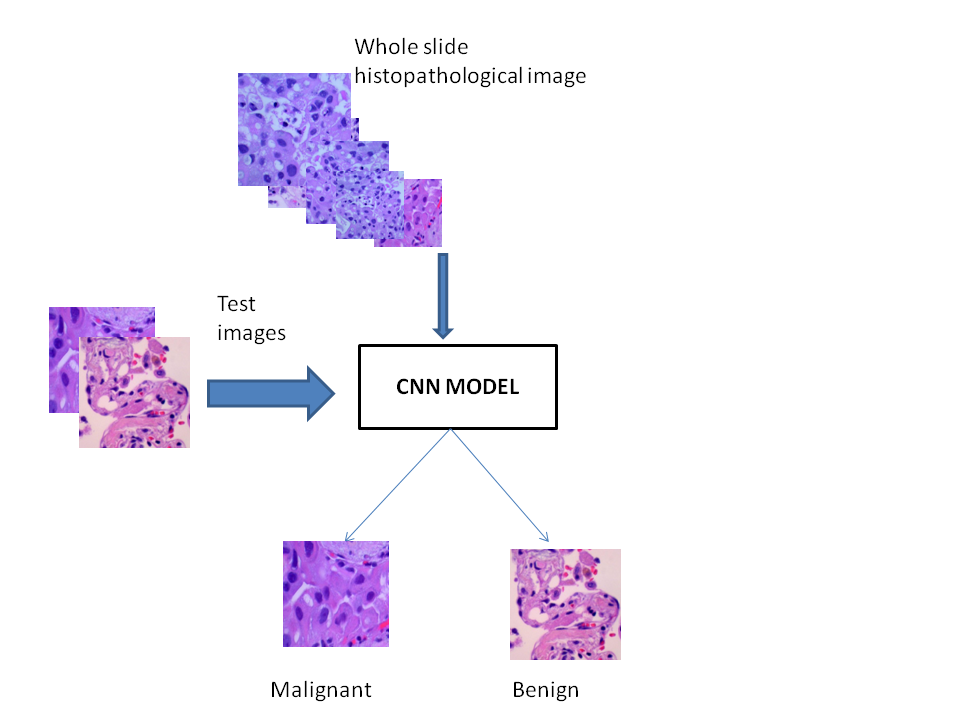
\includegraphics[width=10cm, height=7cm]{./figures/pic1a.png}}
\caption{Binary Classification of whole slide histopathological images}
\label{fig9}
\end{figure}
\subsubsection{Categorical Classification}
The proposed classification system classifies the lung cancer types into adenocarcinoma, squamous cell carcinoma and benign. We have used categorical cross entropy as loss function. The module diagram for the proposed system is shown in Figure \ref{fig10}.\newline
\begin{figure}[htbp]
\centerline{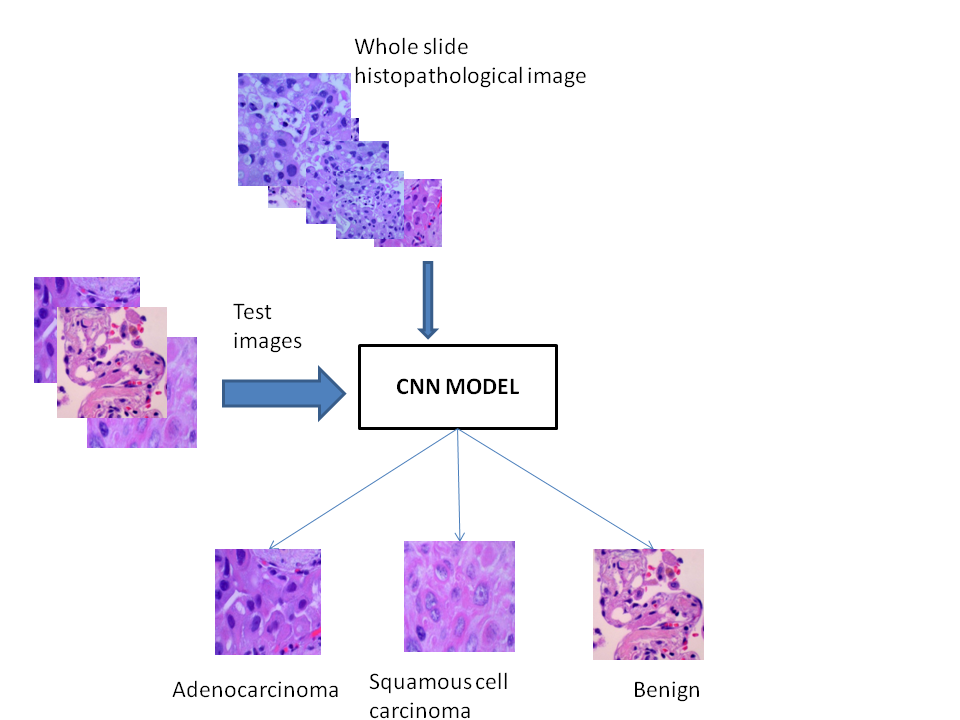
\includegraphics[width=10cm, height=7cm]{./figures/pic2a.png}}
\caption{Categorical Classification of whole slide histopathological images}
\label{fig10}
\end{figure}

\subsection{Lung Cancer Classification From Whole Slide Histopathological Images}
\newline
\textbf{Binary Classification}
%


The model is trained for totally 8000 images, where 4000 samples are malignant sub-types and 4000 samples are benign. The proposed classification system classifies the given sample into malignant and benign. The test set contains a total of totally 2000 images, 1000 images of malignant sub-type and 1000 images are of benign type samples. The confusion matrix is shown in Table \ref{table1}. We have inferred the following information from the confusion matrix \ref{table1}, that is the model has classified all the images correctly.
\begin{table}
\begin{center}
\begin{tabular}[scale=2.0]{ | c |c  |c  | }
  \hline        
  &  &\\
  Types  & Benign & Malignant  \\
  & & \\
   \hline
   &  & \\
  Benign & 1000  &  0   \\ 
  & & \\
  \hline
  &  & \\
  Malignant  & 0 &    1000   \\
  & & \\
  \hline  
\end{tabular}
\caption{Confusion matrix for Binary classification from whole slide histopathological images}
\label{table1}
\end{center}
\end{table}
\newpage






\textbf{Categorical Classification}
%


The proposed classification module classifies the given image sample into adenocarcinoma, squamous cell carcinoma and benign. The model is trained for totally 12,000 images, where each class has 4000 samples. The test set contains totally 3000 samples, where each class has 1000 images.The confusion matrix is shown in Table \ref{table2}. We have inferred the following information from the confusion matrix \ref{table2}, for the class adenocarcinoma the model has classified 991 images correctly out of 1000 images, for the class squamous cell carcinoma the model has classified 983 images out of 1000 images and for the class benign the model has classified all the 1000 images correctly. From this we can say that the model has confused between the malignant sub-types and correctly classifying the benign type.

\begin{table}
\begin{center}
\begin{tabular}[scale=1.4]{ | c | c | c | c | }
  \hline        
   & & &\\
   Types & ADC & Benign & SCC \\
   & & & \\
   \hline
   & & &\\
   ADC & 991  & 1 & 8 \\
   & & &\\
   \hline
   & & &\\
   Benign & 0 & 1000 & 0 \\
   & & &\\
   \hline
   & & &\\
   SCC & 27 & 0 & 983 \\
   &  & &\\
  
  \hline  
\end{tabular}
\caption{Confusion matrix for Categorical classification from whole slide histopathological images }
\label{table2}
\end{center}
\end{table}




\subsection{Lung Cancer Classification From Segmented Nucleus Using Deep Learning}
\subsubsection{Threshold Based Segmentation}
The input for this module is segmented nucleus from the whole slide histopathological images. The nuclei are segmented based on the threshold value.

\newline
\textbf{Binary Classification}
%


This module classifies the given sample into malignant vs benign. The module is trained for 8000 images(each class 4000 images). The test set contains totally 2000 images (each class 1000 images). The confusion matrix is shown in Table \ref{table3}. We have inferred the following information from the confusion matrix \ref{table3}, for the benign class the model has classified 976 images out 1000 images and for the malignant class the model has classified all the images correctly. 

\begin{table}
\begin{center}
\begin{tabular}[scale=2.0]{ | c |c  |c  | }
  \hline    
  &  &\\
  Types  & Benign & Malignant  \\
  & & \\
   \hline
   &  & \\
  Benign & 976  &  24   \\ 
  & & \\
  \hline
  &  & \\
  Malignant  & 0 &    1000   \\
  & & \\
  \hline  
\end{tabular}
\caption{Confusion matrix for Binary classification from segmented nuclei using thresholding}
\label{table3}
\end{center}
\end{table}
\newpage


\newpage
%
\newpage
\textbf{Categorical Classification}\newline
The proposed classification system classifies the given samples into adenocarcinoma, squamous cell carcinoma, benign. This module is trained for 12,000 images (each class 4000 images). The test set contains a total of 3000 samples (each class 1000 samples).The confusion matrix is shown in Table \ref{table4}. We have inferred the following information from the confusion matrix \ref{table4}, for the class adenocarcinoma the model has classified 974 images correctly out of 1000 images, for the class squamous cell carcinoma the model has classified all the images correctly and for the class benign the model has classified all the images correctly.

\begin{table}
\begin{center}
\begin{tabular}[scale=1.4]{ | c | c | c | c | }
  \hline        
   &  & &\\
   Types & ADC & Benign & SCC  \\
    &  & &\\
   \hline        
   &  & &\\
   ADC & 974  & 0 & 26 \\
   & & &\\
   \hline
   & & &\\
   Benign & 0 & 1000 & 0 \\
   & & &\\
   \hline
   & & &\\
   SCC & 0 & 0 & 1000 \\
   &  & &\\
  
  \hline  
\end{tabular}
\caption{Confusion matrix for Categorical classification from segmented nuclei using thresholding }
\label{table4}
\end{center}
\end{table}

\subsubsection{Color Based Segmentation}
The proposed module takes the segmented nuclei as input and classifies them. Here the nucleus are segmented using color based technique.

\newline
\textbf{Binary Classification}
%


This module classifies the given sample into malignant vs benign. The module is trained for 8000 images(each class 4000 images). The test set contains totally 2000 images (each class 1000 images). The confusion matrix is shown in Table \ref{table5}. We have inferred the following information from the confusion matrix \ref{table5}, for the malignant class the model has classified 951 images correctly out of 1000 images and for the class benign the model has classified all the 1000 images correctly.

\begin{table}
\begin{center}
\begin{tabular}[scale=2.0]{ | c |c  |c  | }
  \hline        
  &  &\\
  Types  & Benign & Malignant  \\
  & & \\
   \hline
   &  & \\
  Benign & 1000  &  0   \\ 
  & & \\
  \hline
  &  & \\
  Malignant  & 49 &  951   \\
  & & \\
  \hline  
\end{tabular}
\caption{Confusion matrix for Binary classification color based segmented nuclei}
\label{table5}
\end{center}
\end{table}
\newpage



\newline
\textbf{Categorical Classification}
%

\begin{comment}
\textbf{Categorical Classification}\newline
The proposed classification system classifies the given samples into adenocarcinoma, squamous cell carcinoma, benign. This module is trained for 12,000 images (each class 4000 images). The test set contains a total of 3000 samples (each class 1000 samples).The confusion matrix is shown in Table \ref{table4}. We have inferred the following information from the confusion matrix \ref{table4}, for the class adenocarcinoma the model has classified 974 images correctly out of 1000 images, for the class squamous cell carcinoma the model has classified all the images correctly and for the class benign the model has classified all the images correctly.

\begin{table}
\begin{center}
\begin{tabular}[scale=1.4]{ | c | c | c | c | }
  \hline        
   &  & &\\
   Types & ADC & Benign & SCC  \\
    &  & &\\
   \hline        
   &  & &\\
   ADC & 974  & 0 & 26 \\
   & & &\\
   \hline
   & & &\\
   Benign & 0 & 1000 & 0 \\
   & & &\\
   \hline
   & & &\\
   SCC & 0 & 0 & 1000 \\
   &  & &\\
  
  \hline  
\end{tabular}
\caption{Confusion matrix for Categorical classification from segmented nuclei using thresholding }
\label{table4}
\end{center}
\end{table}

\subsubsection{Color Based Segmentation}
Normally, the histopathological images are stained  using H&E. Hence, it is possible to filter out the nuclei from the Whole Slide Images based on the hue values. The segmented nuclei so obtained, are classified using the proposed CNN model. 

\textbf{Binary Classification}

This module classifies the given sample into malignant vs benign. The module is trained for 8000 images(each class 4000 images). The test set contains totally 2000 images (each class 1000 images). The confusion matrix is shown in Table \ref{table5}. We have inferred the following information from the confusion matrix \ref{table5}, for the malignant class the model has classified 951 images correctly out of 1000 images and for the class benign the model has classified all the 1000 images correctly.

\begin{table}
\begin{center}
\begin{tabular}[scale=2.0]{ | c |c  |c  | }
  \hline        
  &  &\\
  Types  & Benign & Malignant  \\
  & & \\
   \hline
   &  & \\
  Benign & 1000  &  0   \\ 
  & & \\
  \hline
  &  & \\
  Malignant  & 49 &  951   \\
  & & \\
  \hline  
\end{tabular}
\caption{Confusion matrix for Binary classification color based segmented nuclei}
\label{table5}
\end{center}
\end{table}




\textbf{Categorical Classification}


The proposed classification system classifies the given samples into adenocarcinoma, squamous cell carcinoma, benign. This module is trained for 12,000 images (each class 4000 images). The test set contains a total of 3000 samples (each class 1000 samples).The the confusion matrix is shown in Table \ref{table6}. We have inferred the following information from the confusion matrix
(Table \ref{table6}), for the class adenocarcinoma the model has classified 877 images correctly out of 1000 images, for the class squamous cell carcinoma the model has classified 672 images out of 1000 images and for the class benign the model has classified all the 1000 images correctly. From this we can say that the model has confused between the malignant sub-types and correctly classifying the benign type.

\begin{table}
\begin{center}
\begin{tabular}[scale=1.3]{ | c | c | c | c |}
  \hline        
   &  & &\\
   Types & ADC  & Benign & SCC  \\
    &  & &\\
    \hline        
   &  & &\\
   ADC & 877  & 22 & 101 \\
   & & &\\
   \hline
   & & &\\
   Benign & 0 & 1000 & 0 \\
   & & &\\
   \hline
   & & &\\
   SCC & 303 & 25 & 672 \\
   &  & & \\
  
  \hline  
\end{tabular}
\caption{Confusion matrix for Categorical classification from color based segmented nuclei}
\label{table6}
\end{center}
\end{table}





\begin{figure}[htbp]
\centerline{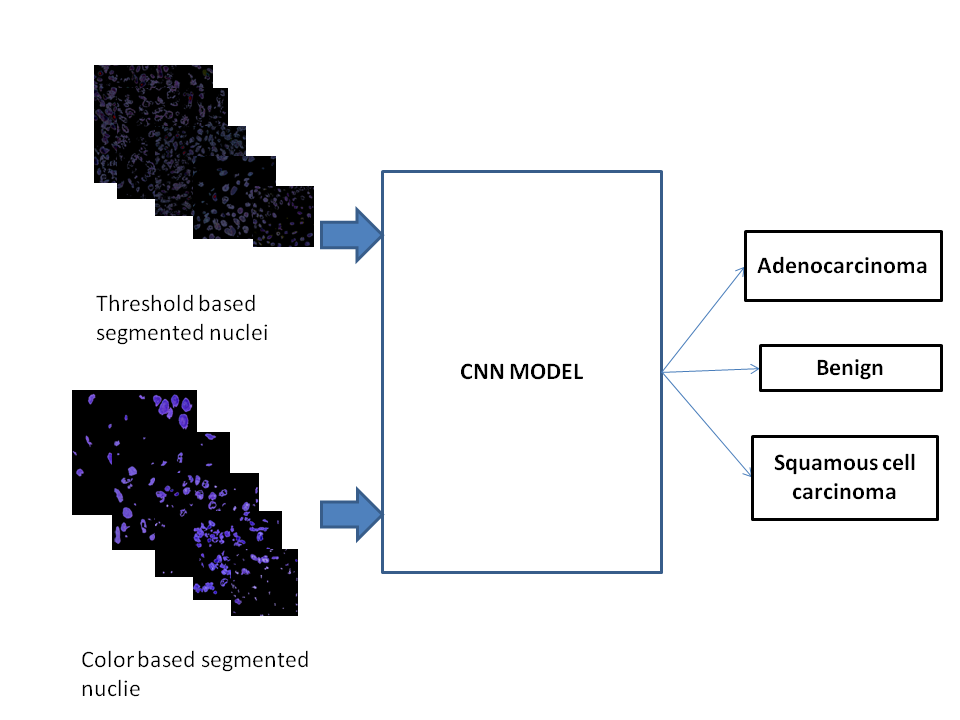
\includegraphics[width=8cm, height=7cm]{./figures/categorical.png}}
\caption{Categorical classification of lung cancer types from the segmented nuclei}
\label{categorical}
\end{figure}
\end{comment}

The proposed classification system classifies the given samples into adenocarcinoma, squamous cell carcinoma, benign. This module is trained for 12,000 images (each class 4000 images). The test set contains a total of 3000 samples (each class 1000 samples).The the confusion matrix is shown in Table \ref{table6}. We have inferred the following information from the confusion matrix
(Table \ref{table6}), for the class adenocarcinoma the model has classified 877 images correctly out of 1000 images, for the class squamous cell carcinoma the model has classified 672 images out of 1000 images and for the class benign the model has classified all the 1000 images correctly. From this we can say that the model has confused between the malignant sub-types and correctly classifying the benign type.

\begin{table}
\begin{center}
\begin{tabular}[scale=1.3]{ | c | c | c | c |}
  \hline        
   &  & &\\
   Types & ADC  & Benign & SCC  \\
    &  & &\\
    \hline        
   &  & &\\
   ADC & 877  & 22 & 101 \\
   & & &\\
   \hline
   & & &\\
   Benign & 0 & 1000 & 0 \\
   & & &\\
   \hline
   & & &\\
   SCC & 303 & 25 & 672 \\
   &  & & \\
  
  \hline  
\end{tabular}
\caption{Confusion matrix for Categorical classification from color based segmented nuclei}
\label{table6}
\end{center}
\end{table}

\subsection{Result Analysis}
The overall performance of an entire system has been tabulated in (Table \ref{result analysis}). The binary classification of lung cancer types from the whole slide histopathological images have got highest accuracy of 100\%. From this we inferred that the module distinguish between benign and malignant type cancer cells more accurately. The categorical classification of lung cancer types from the color based segmented nuclei have got accuracy of 84\%. The categorical classification have got lesser accuracy when compared to binary classification, because the module found difficult to distinguish between malignant sub-types (Adenocarcinoma and Squamous cell carcinoma).
\begin{table}[h]
\footnotesize
\begin{center}
\begin{tabular}{|c|c|c|}
  \hline        
   &  & \\
   \textbf{Classification Modules}  & \textbf{Binary Classification} & \textbf{Categorical Classification} \\
   & & \\
   \hline
   & & \\
   Lung cancer classification 
   from whole slide 
    &  100\% & 99\% \\
    Histopathological images & &\\
   & & \\
   \hline
   & & \\
   Lung cancer classification
   from  & 98\% & 99\% \\
   segmented nuclei
   (Threshold based) & &\\
   &  & \\
   \hline
   & & \\
   Lung cancer classification 
   from  & 97\% & 84\%  \\
   segmented Nuclei
   (Color based) & & \\
   &  & \\
  
  \hline  
\end{tabular}
\caption{Result Analysis}
\label{result analysis}
\end{center}
\end{table}


\section*{Conclusion}
Lung cancer classification from histopathological images using deep learning was proposed. CNN was considered as the baseline for our proposed system of lung cancer classification, because of its automatic feature extraction, which reduces the error and increase the overall system performance. We have proposed two methods for lung cancer classification from the histopathological images. The first method classifies the lung cancer types from the whole slide histopathological images. 

The lung cancer mainly affects the nucleus of the tissue, therefore the cancer cells are mainly found in the nucleus. The second module classifies the lung cancer types from the segmented nucleus. The nucleus from the whole slide histopathological images were segmented using two different method, one is based on the the threshold value and the other one is based on the color of the nucleus. The lung cancer classification from whole slide histopathological images got an accuracy of 99\%, we have obtained an accuracy of 99\% and 84\% from our proposed classification method after segmenting the nucleus using threshold based and color based. 

Through this, we inferred that Convolution Neural Network has potential to perform lung cancer classification on both whole slide histopathological images and nucleus segmented from the image tissues. This work can be further be extended by performing nucleus segmentation using deep learning architecture(U-net). This may increase the accuracy of the classification based on nucleus segmentation. 
%\section*{References}



\bibliographystyle{spmpsci}   
\bibliography{ref_tencon_2019}   



\end{document}
